%12_graphs_two.tex
%notes for the course PandA2 COMS10001 taught at the University of Bristol
%2016-7 Conor Houghton conor.houghton@bristol.ac.uk

%To the extent possible under law, the author has dedicated all copyright 
%and related and neighboring rights to these notes to the public domain 
%worldwide. These notes are distributed without any warranty. 

\documentclass[11pt,a4paper]{scrartcl}
\typearea{12}
\usepackage{graphicx}
\usepackage{listings}
\usepackage{tikz}
%\usepackage{tikz-qtree}                                                        
\usetikzlibrary{positioning}
\lstset{language=C}
\pagestyle{headings}
\markright{COMS10001 - PandA2 12\_graphs\_two - Conor}
\begin{document}

\subsection*{12- graphs two\footnote{\texttt{http://github.com/conorhoughton/COMS10001}} - DRAFT}

In these notes we will learn about two constructive algorithms; the
first, Fleury's Algorithm, allows an Eulerian path to be constructed
if one exists and the second, Dijkstra's Algorithm, a very famous and
useful algorithm, allows us to find the shortest path through a
weighted graph. We won't look at a formal proof in either case, but
for both the algorithms are compelling enough that it is reasonably
clear how a proof might work.

\subsubsection*{Fleury's algorithm}


\begin{figure}
\begin{center}
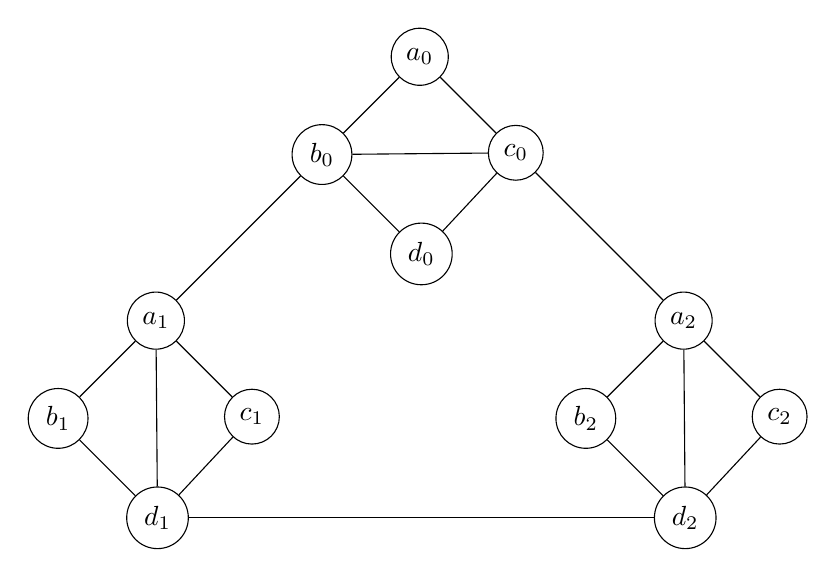
\begin{tikzpicture}
\node[draw,circle](a){$a_0$};
\node[draw,circle, below left= 1cm of a](b){$b_0$};
\node[draw,circle, below right =1cm of a](c){$c_0$};
\node[draw,circle, below right = 1cm of b](d){$d_0$};
\path (a) edge (b);
\path (a) edge (c);
\path (b) edge (d);
\path (c) edge (d);
\path (b) edge (c);

\node[draw,circle,below left=4cm of a](a1){$a_1$};
\node[draw,circle, below left= 1cm of a1](b1){$b_1$};
\node[draw,circle, below right =1cm of a1](c1){$c_1$};
\node[draw,circle, below right = 1cm of b1](d1){$d_1$};
\path (a1) edge (b1);
\path (a1) edge (c1);
\path (b1) edge (d1);
\path (c1) edge (d1);
\path (a1) edge (d1);


\node[draw,circle,below right=4cm of a](a2){$a_2$};
\node[draw,circle, below left= 1cm of a2](b2){$b_2$};
\node[draw,circle, below right =1cm of a2](c2){$c_2$};
\node[draw,circle, below right = 1cm of b2](d2){$d_2$};
\path (a2) edge (b2);
\path (a2) edge (c2);
\path (b2) edge (d2);
\path (c2) edge (d2);
\path (a2) edge (d2);

\path (d1) edge (d2);
\path (b) edge (a1);
\path (c) edge (a2);



\end{tikzpicture}
\end{center}
\caption{A graph that usefully illustrates Fleury's algorithm. \label{fig:graph}}
\end{figure}




Imagine trying to find an Eulerian cycle for the graph in
Fig.~\ref{fig:graph}, but without thinking about it too hard; say you
start at $a_0$ and go to $b_0$ before heading off for $a_1$, then
$b_1$ and $d_1$ before going hog-wild and going on to $d_2$, the
situation you find yourself in is illustrated in
Fig.~\ref{fig:graph_hw}; it is clear the situation is hopeless, there
is no way to return to the subscript-1 group of nodes to traverse the
edges between $a_1$ and $d_1$, $a_1$ and $c_1$ and $d_1$ and
$c_1$. These should have been finished up before leaving for the
subscript-2 nodes. The sequence $a_0b_0a_1d_1a_1c_1d_1d_2$, but even
if the subscript-2 nodes are all carefully visited,
$d_2b_2a_2c_2d_2a_2$ before returning to the subscript-0 nodes,
$a_2c_0$ it is still possible to mess ip by returning to $a_0$ before
visiting the edges $c_0d_0b_0c_0$.

Playing with this example shows that the problem is with creating
\lq{}islands\rq{}, a node, or group of nodes, you can't return to
because all the links to them have been used up. At this point it is
useful to define a \textsl{bridge}, a bridge is an edge which, if it
was removed, would leave the graph disconnected; examples are given in
Fig.~\ref{fig:bridges}. Now imagine removing the edges as you traverse
them, if you remove a bridge then you cannot return to the nodes left
behind, so when trying to walk an Eulerian path it is important not to
remove bridges if there are still edges to walk. This is basically
Fleury's algorithm, it says that you should never choose a bridge if
there is a choice, this is summarized in Table~\ref{table:fleury}.

\begin{table}
\begin{itemize}
\item As you traverse each edge remove it.
\item If a node has an edge that isn't a bridge take that.
\end{itemize}
\caption{Fleury's algorithm \label{table:fleury}}
\end{table}
  
\begin{figure}
\begin{center}
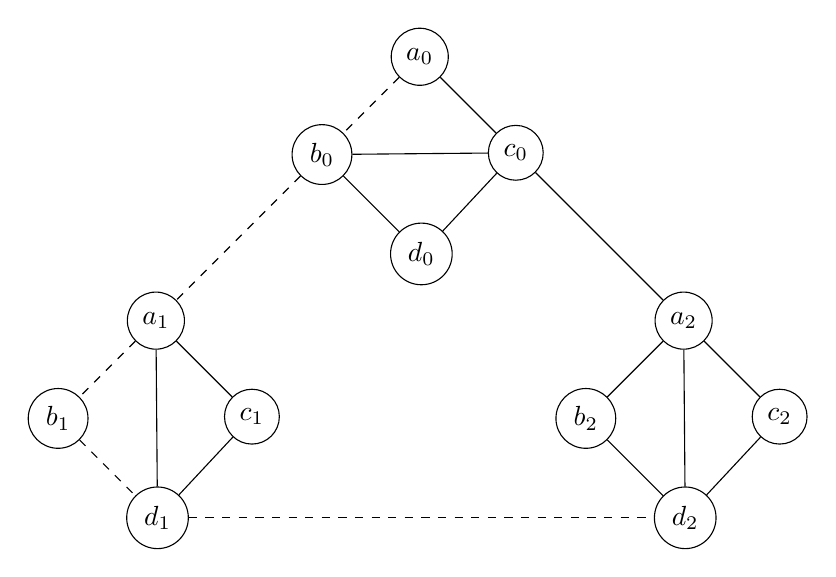
\begin{tikzpicture}
\node[draw,circle](a){$a_0$};
\node[draw,circle, below left= 1cm of a](b){$b_0$};
\node[draw,circle, below right =1cm of a](c){$c_0$};
\node[draw,circle, below right = 1cm of b](d){$d_0$};
\path (a) edge[dashed] (b);
\path (a) edge (c);
\path (b) edge (d);
\path (c) edge (d);
\path (b) edge (c);

\node[draw,circle,below left=4cm of a](a1){$a_1$};
\node[draw,circle, below left= 1cm of a1](b1){$b_1$};
\node[draw,circle, below right =1cm of a1](c1){$c_1$};
\node[draw,circle, below right = 1cm of b1](d1){$d_1$};
\path (a1) edge[dashed] (b1);
\path (a1) edge (c1);
\path (b1) edge[dashed] (d1);
\path (c1) edge (d1);
\path (a1) edge (d1);


\node[draw,circle,below right=4cm of a](a2){$a_2$};
\node[draw,circle, below left= 1cm of a2](b2){$b_2$};
\node[draw,circle, below right =1cm of a2](c2){$c_2$};
\node[draw,circle, below right = 1cm of b2](d2){$d_2$};
\path (a2) edge (b2);
\path (a2) edge (c2);
\path (b2) edge (d2);
\path (c2) edge (d2);
\path (a2) edge (d2);

\path (d1) edge[dashed] (d2);
\path (b) edge[dashed] (a1);
\path (c) edge (a2);



\end{tikzpicture}
\end{center}
\caption{A bad start to finding an Eulerian path, the edges already traversed are dashed.\label{fig:graph_hw}}
\end{figure}





\begin{figure}
\begin{center}
\begin{tikzpicture}
\node[draw,circle](a){};
\node[draw,circle, below left= 1cm of a](b){};
\node[draw,circle, below right =1cm of a](c){};
\node[draw,circle, below right = 1cm of b](d){};
\path (a) edge (b);
\path (a) edge (c);
\path (b) edge (d);
\path (c) edge (d);
\path (b) edge (c);

\node[draw,circle,right=4cm of a](a1){};
\node[draw,circle, below left= 1cm of a1](b1){};
\node[draw,circle, below right =1cm of a1](c1){};
\node[draw,circle, below right = 1cm of b1](d1){};
\path (a1) edge (b1);
\path (a1) edge (c1);
\path (b1) edge (d1);
\path (c1) edge (d1);
\path (a1) edge (d1);


\node[draw,circle,right=4cm of a1](a2){};

\path (a1) edge[dashed] (a2);
\path (c) edge[dashed] (b1);

\end{tikzpicture}
\end{center}
\caption{The two dashed edges are bridges since deleting either of them would make the graph disconnected. \label{fig:bridges}}
\end{figure}

\subsubsection*{Dijkstra's algorithm}

The problem Dijkstra's algorithm solves is how to find the shortest path through a weighted graph. Consider the graph in Fig

\begin{figure}
\begin{center}
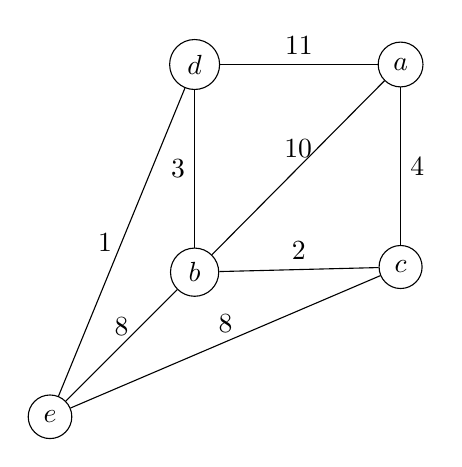
\begin{tikzpicture}
\node[draw,circle](a){$a$};
\node[draw,circle, below      =2cm of a](c){$c$};
\node[draw,circle, left = 2cm of a](d){$d$};
\node[draw,circle, below = 2 cm of d](b){$b$};
\node[draw,circle, below left = 2 cm of b](e){$e$};
\path (a) edge node[above]{10} (b);
\path (a) edge node[right]{4} (c);
\path (b) edge node[left]{3} (d);
\path (a) edge node[above]{11} (d);
\path (b) edge node[above]{2} (c);
\path (b) edge node[above]{8} (e);
\path (d) edge node[left]{1} (e);
\path (c) edge node[above]{8} (e);
\end{tikzpicture}
\end{center}
\end{figure}


\begin{figure}
\begin{center}
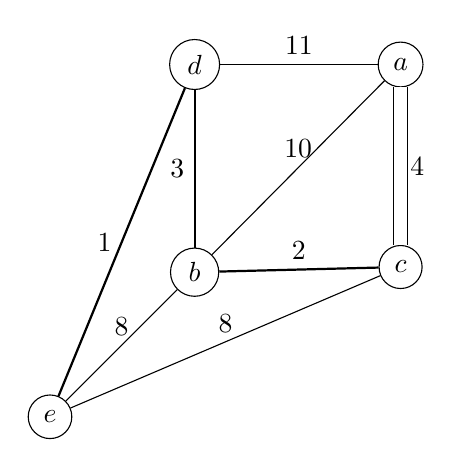
\begin{tikzpicture}
\node[draw,circle](a){$a$};
\node[draw,circle, below      =2cm of a](c){$c$};
\node[draw,circle, left = 2cm of a](d){$d$};
\node[draw,circle, below = 2 cm of d](b){$b$};
\node[draw,circle, below left = 2 cm of b](e){$e$};
\path (a) edge node[above]{10} (b);
\draw[double, double distance between line centers=0.5em] (a) -- node[right]{4} (c);
\path (b) edge[thick] node[left]{3} (d);
\path (a) edge node[above]{11} (d);
\path (b) edge[thick] node[above]{2} (c);
\path (b) edge node[above]{8} (e);
\path (d) edge[thick] node[left]{1} (e);
\path (c) edge node[above]{8} (e);
\end{tikzpicture}
\end{center}
\end{figure}



\end{document}
